\documentclass[../EngineeringJournal_CDavis.tex]{subfiles}

\begin{document}

%%%%%%%%%%%%%%%%%%%%%%%%%%%%%%%%%%%%%%%%%%%%%%%%%%%%%
%%%%%%%%%%%%%%%%%%%%%%%%%%%%%%%%%%%%%%%%%%%%%%%%%%%%%

\chapter[Configuring IPv4 Static]{Configuring IPv4\linebreak[1] Static Routes \hspace*{\fill}{Feb 8, 2020}}
\noindent\textbf{{Packet Tracer Lab 6} \hspace*{\fill}{\textbf{CIT 167}}}\linebreak[1]
{{Spring 2020} \hspace*{\fill}{Chaz Davis}}                             
%===================================
%===================================

\hspace{0.2cm}
\begin{tcolorbox}[width=6.3in]
\scriptsize 
- Important Concepts for the Lab
  \begin{itemize}
    \item{Recursive static route}
      \subitem{}a route whose next hop and destination network 
	are covered by another learned route in the 
	Routing Information Database (RIB).
      \subitem{} Such static routes cannot be installed in the 
	  RIB because they are considered redundant routes. 
    \item{Directly Connected Static Route}     
      \subitem{} A directly connected static route is one that 
      uses the exit interface to forward traffic to the 
      intended destination.
        \subitem{} This is in contrast to the recursive static route
	which used the next hop IP address of the router 
	along the path to the destination
    \item{Loopback} 
        \subitem{} A loopback interface is a logical, virtual interface in 
	a cisco router.
	\subitem{} A loopback interface is not a physical interface like 
	  Fast Ethernet or Gigabit Ethernet interface. 
    \item{A loopback interface has many uses}
        \subitem{} Loopback interface's  IP Address determines a routers OSPF
	Router ID.
	\subitem{} A loopback interface is always up and allows Border
	  Gateway Protocol (BGP) neighborship between two routers to stay
	  up even if one of the outbound physical interfaces is down.
  \end{itemize}
\end{tcolorbox}
\hspace{0.2cm}
\normalsize  

\newpage

%===================================
\mysection{\textbf{Part 1: Setting up the topology}}
\mysubsection{1}{Cabling the Network}\\
I've configured the network with two routers, 2 switches, and 2 pcs as seen in
Fig.~\ref{Topo6}.
\begin{figure}[!hbt]
  \centering
  \subfloat[Cabling the topology]{\label{Topo6}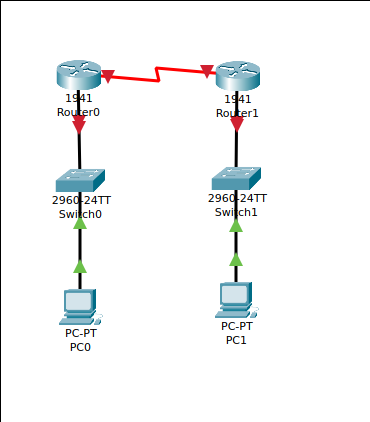
\includegraphics[width=.45\linewidth]{Figures/2020-02-07-113805_370x422_scrot.png}}\par
\end{figure}

\noindent\mysubsection{2}{Initialization}\\
I flipped the switches and restarted the routers and switches.

%===================================
\mysection{\textbf{Part 2: Configuring Basic Device Settings}}

\mysubsection{1}{Configuring the PC Interfaces}\\
I configured the PCs according to the table. As you can see in
Fig.~\ref{NetConfig6}\subref{NetConfig6PCA} and
Fig.~\ref{NetConfig6}\subref{NetConfig6PCB} on Pg.~\pageref{NetConfig6}.


\noindent\mysubsection{2}{Verify the LANs}\\
Next, I ran commands on the routers to configure the device names, setup DNS lookup,
added passwords, and then ran the configuration and startup styles.

\noindent\mysubsection{3}{Configuring IP settings on the routers}\\
Finally, I configured the ip addresses on the routers and set up the static routing
tables for the addresses. See Fig.~\ref{NetConfig6}\subref{NetConfig6R3} and
Fig.~\ref{NetConfig6}\subref{NetConfig6R1} on Pg.~\pageref{NetConfig6}.

\begin{figure}[!hbt]\centering
  \subfloat[PC-A IP config]{\label{NetConfig6PCA}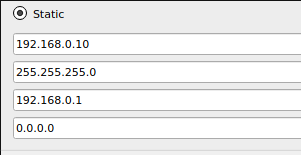
\includegraphics[width=.43\linewidth]{Figures/2020-02-07-115624_301x155_scrot.png}}\hfill
  \subfloat[PC-B IPConfig]{\label{NetConfig6PCB}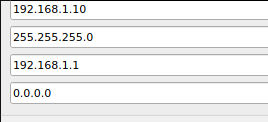
\includegraphics[width=.49\linewidth]{Figures/2020-02-07-115706_268x122_scrot.png}}\par
  \subfloat[The network now]{\label{NEtConfig6Network}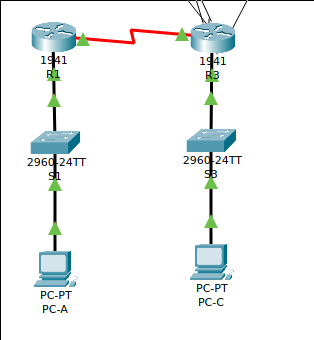
\includegraphics[width=.45\linewidth]{Figures/2020-02-07-115938_314x340_scrot.png}}\par
  \subfloat[Router 3 config]{\label{NetConfig6R3}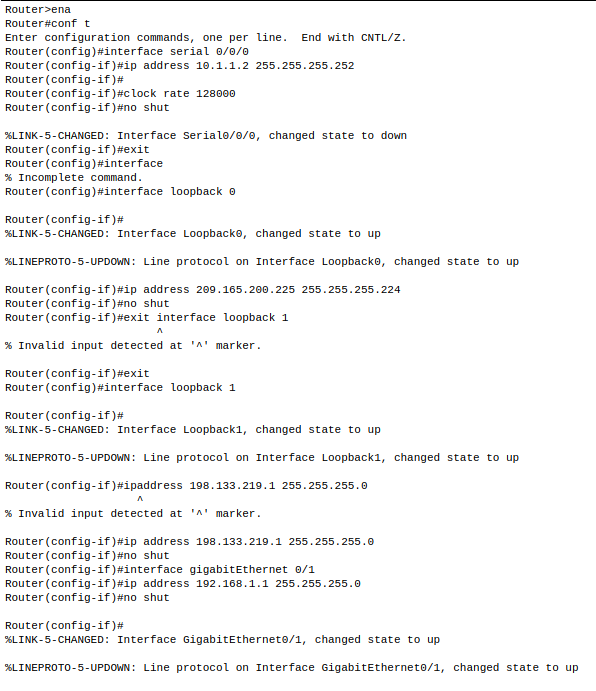
\includegraphics[width=.45\linewidth]{Figures/2020-02-07-115250_596x691_scrot.png}}\hfill
  \subfloat[router 1 config]{\label{NetConfig6R1}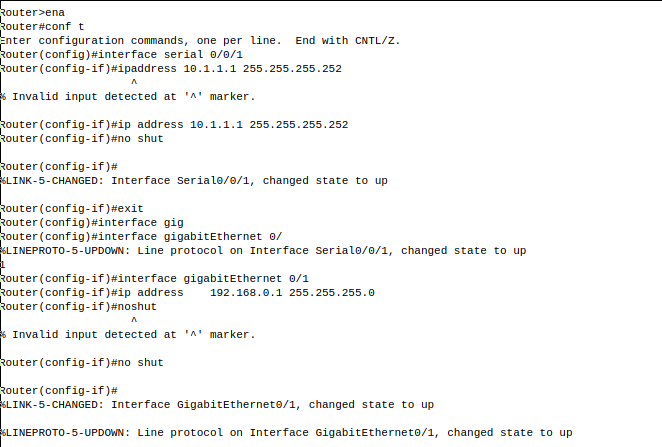
\includegraphics[width=.49\linewidth]{Figures/2020-02-07-115509_662x447_scrot.png}}\par
\caption{Configuring the network interfaces}\label{NetConfig6}
\end{figure}


\clearpage 

\noindent\mysubsection{4}{Verify Connectivity of LANs}\\
I tested conectivity by pinging from each PC. I was able to ping from PC to router
but from PC-A I was ubnable to reach PC-C or either loopback. See Fig.~\ref{LanConnect6}\subref{LanConnect6pcA}.
and Fig.~\ref{LanConnect6}\subref{LanConnect6pcC} on Pg.~\pageref{LanConnect6}. 


\begin{figure}[!hbt]\centering
\subfloat[Pinging the default gateway from PC-A\\ Pinging PC-C, Lo0, and Lo1 from PC-A]{\label{LanConnect6pcA}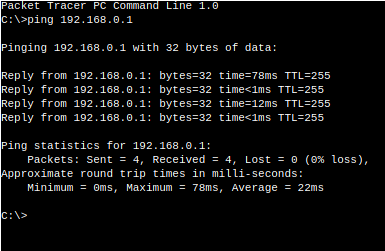
\includegraphics[width=.40\linewidth]{Figures/2020-02-08-154606_385x251_scrot.png}}\hfill
\subfloat[Pinging the default gateway from PC-C]{\label{LanConnect6pcC}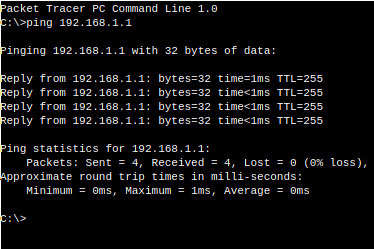
\includegraphics[width=.40\linewidth]{Figures/2020-02-08-154617_374x249_scrot.png}}\par 
\subfloat[Pinging S0/0/0 and R3 from R1]{\label{LanConnect6R1}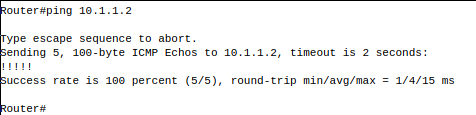
\includegraphics[width=.45\linewidth]{Figures/2020-02-08-154731_476x115_scrot.png}}
\caption{Verifying Connections between devices on the network}\label{LanConnect6}
\end{figure}

\clearpage

%===================================
\mysection{\textbf{Part 3: Configure Static Routes}}
\mysubsection{1}{Configure recursive static route}\\
I went to R1 and entered the command 
{\scriptsize{\verb$ip route 192.168.1.0 255.255.255.0 10.1.1.2$}\normalsize} 
in to the command line.\\
The new {\scriptsize{\verb$show ip route$}\normalsize} shows us the static
routing configuration.\\
In the last line  we see {\scriptsize{\verb$S 192.168.1.0/24 [1/0] via 10.1.1.2$}\normalsize} .

\noindent\mysubsection{2}{Configure directly connected static route}\\
I went to R3 and 
entered {\scriptsize{\verb$ip route 192.168.0.0 255.255.255.0 serial 0/0/0$}\normalsize}.\\
When I run the {\scriptsize{\verb$show ip route$}\normalsize} command from R3 we can now see the static exit interface in the line {\scriptsize{\verb$S    192.168.0.0/24 is directly connected, Serial0/0/0$}\normalsize}.


\noindent\mysubsection{3}{Configure Static Route}\\
I went to R1 and ran {\scriptsize{\verb$ip route 198.133.219.0 255.255.255.0 serial 0/0/1$}\normalsize}.


\noindent\mysubsection{4}{Remove static Routes for Loopback}\\
I went to R1 and 
ran {\scriptsize{\verb$ip route 209.165.200.224 255.255.255.224 10.1.1.2$}\normalsize}\\
and now we can see with the lines: 
\begin{mdframed}
\scriptsize
\begin{verbatim}

S    198.133.219.0/24 is directly connected, Serial0/0/1
     209.165.200.0/27 is subnetted, 1 subnets
S       209.165.200.224/27 [1/0] via 10.1.1.2
\end{verbatim}
\normalsize
\end{mdframed}


That we are correctly configured.

\clearpage

%===================================
\mysection{\textbf{Part 4: Configure and verify the default route}}
I went to R1 and entered 
{\scriptsize{\verb$ip route 0.0.0.0 0.0.0.0$}\normalsize}.\\
I the went to PC-A and Pinged 209.165.200.225 see
Fig.~\ref{verify6}\subref{verify6ping1}\\
Lastly, I pinged 198.133.219.1 from PC-A. See Fig.~\ref{verify6}\subref{verify6ping2}

\begin{figure}[!hbt]\centering
\subfloat[Pinging PC-C from PC- A]{\label{verify6ping1}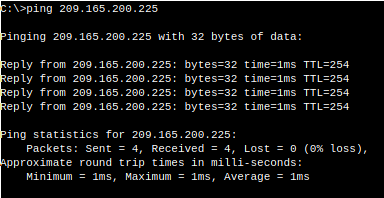
\includegraphics[width=.45\linewidth]{Figures/2020-02-08-171935_384x198_scrot.png}}\hfill
\subfloat[Pinging R1 from PC-A]{\label{verify6ping2}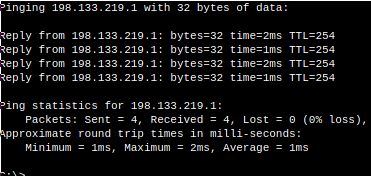
\includegraphics[width=.45\linewidth]{Figures/2020-02-08-171948_371x176_scrot.png}}\par 
\caption{Verifying the default routes}\label{verify6}
\end{figure}

\clearpage


%===================================
\mysection{\textbf{Reflection}}
If we added a new network we could run\\
{\scriptsize{\verb$ip route 192.168.3.0 255.255.255.0 s0/0/0$}\normalsize}\\
{\scriptsize{\verb$ip route 192.168.3.0 255.255.255.0 10.1.1.1$}\normalsize}
from R3\\
With a recursive static route perform lookups in the routing table before forwarding
the packets. With a directly connected static route, the exit-interface  parameter is
specified, which allows the route to resolve a forwarding decision in one
lookup.\\
A default gateway tells the device to contact the next hop of the default route if
they don't have a more specific route. Without a default route, a router will drop a
request for a network that is not in its routing table and send ICMP Destination
unreachable.



%===================================

\end{document}
